%% --------------------------------------------------------------------------
% LaTeX template for the XLII CILAMCE-PANACME.
%
% This latex document tries to copy the Microsoft Word template.
% --------------------------------------------------------------------------
\documentclass[a4paper,10pt]{book}

% PACKAGES USED - packages that need to be previously installed on your computer
\usepackage[lmargin=2.5cm, rmargin=2.5cm, tmargin=2.5cm, bmargin=2.5cm ]{geometry}
\usepackage{graphicx}
\usepackage{times}
\usepackage{indentfirst}
\usepackage{fancyhdr}
\usepackage{titlesec}
\usepackage[english]{babel}
\usepackage{parskip} 
\usepackage{setspace}

%%%%%%%%%%%%%%%%%%%%%%%%%%%%%%%%%%%%%%%%%%%%%%%%%%%%%%%%%%
% GRUMEC
%%%%%%%%%%%%%%%%%%%%%%%%%%%%%%%%%%%%%%%%%%%%%%%%%%%%%%%%%%
%Lagrangian position (inital configuration) vector
\newcommand{\lPosition}{\mathbf{x}}
%Eulerian position (current configuration) vector
\newcommand{\ePosition}{\mathbf{y}}
%Current velocity
\newcommand{\eVelocity}{\dot{\mathbf{y}}}
%Eulerian acceleration (current configuration) vector
\newcommand{\eAccel}{\ddot{\mathbf{y}}}
%rigth Cauchy-Green stretch tensor
\newcommand{\cauchyStretch}{\mathbf{C}}
%Green-Lagrange strain tensor
\newcommand{\greenStrain}{\mathbf{E}}
%Configuration change function
\newcommand{\cChange}{\mathbf{f}}
%Gradient of Configuration change function
\newcommand{\cChangeGrad}{\mathbf{A}}
%Maping to initial
\newcommand{\lMap}{\mathbf{f}_0}
%Gradient of maping to initial
\newcommand{\eMap}{\mathbf{f}_1}
%Green-Lagrange strain rate tensor
\newcommand{\greenStrainRate}{\dot{\mathbf{E}}}
%Lagrangian position (inital configuration) vector
\newcommand{\lPositionh}{\mathbf{x}^h}
%Eulerian position (current configuration) vector
\newcommand{\ePositionh}{\mathbf{y}^h}
%rigth Cauchy-Green stretch tensor
\newcommand{\cauchyStretchh}{\mathbf{C}^h}
%Green-Lagrange strain tensor
\newcommand{\greenStrainh}{\mathbf{E}^h}
%Discretization configuration change function
\newcommand{\cChangeh}{\mathbf{f}^h}
%Discretization mapping function to initial
\newcommand{\mapInih}{\mathbf{f}^{0h}}
%Discretization mapṕing function to final
\newcommand{\mapFinh}{\mathbf{f}^{1h}}
%Gradient of Configuration change function
\newcommand{\cChangeGradh}{\mathbf{A}^h}
%Maping to initial
\newcommand{\cChangeGradfh}{\mathbf{A}^{1h}}
%Maping to initial
\newcommand{\cChangeGradih}{\mathbf{A}^{0h}}
%Maping to initial
\newcommand{\lMaph}{\mathbf{f}^h_0}
%Gradient of maping to initial
\newcommand{\eMaph}{\mathbf{f}^h_1}
%Green-Lagrange strain rate tensor
\newcommand{\greenStrainRateh}{\dot{\mathbf{E}}^h}
%Current spatially discrete velocity
\newcommand{\eVelocityh}{\dot{\mathbf{y}}^h}
%Eulerian acceleration (current configuration) vector
\newcommand{\eAccelh}{\ddot{\mathbf{y}}^h}
%Lagrangian Constitutive Tensor
\newcommand{\lagConst}{\mathbf{D}}
%Discrete Jacobian
\newcommand{\Jh}{J^h}
%Gradient on lagrangian coordinates
\newcommand{\lGrad}{{\pmb{\nabla}}_{\mathbf{x}}}
%Gradient on eulerian coordinates
\newcommand{\eGrad}{{\pmb{\nabla}}_{\mathbf{y}}}

%%%%%%%%%%%%%%%%%%%%%%%%%%%%%%%%%%%%%%%%%%%%%%%%%%%%%%%%%%
% TAFMS
%%%%%%%%%%%%%%%%%%%%%%%%%%%%%%%%%%%%%%%%%%%%%%%%%%%%%%%%%%
\newcommand{\density}{\rho}

\newcommand{\velocity}{\mathbf{u}}

\newcommand{\velocityD}{\mathbf{U}}

\newcommand{\velocityIND}{u}

\newcommand{\stress}{\sigma}

\newcommand{\sstresstensor}{\pmb{\sigma}}

\newcommand{\stresstensor}{\pmb{\sigma}}

%\newcommand{\dyadd}{\otimes}
\newcommand{\dyadd}{ }

\newcommand{\sgn}{\mathrm{sgn}}

\newcommand{\trace}{\mathrm{tr}}

\newcommand{\unittensor}{\mathbf{I}}

\newcommand{\increment}{\varDelta}

\newcommand{\imaginary}{\imath}

\newcommand{\complexspace}{{\mathbb C}}

\newcommand{\mdiffusivity}{\kappa}

\newcommand{\laplacian}{\Delta}

\newcommand{\viscosity}{\mu}

\newcommand{\kviscosity}{\nu}

\newcommand{\diffusivity}{\nu}

\newcommand{\strainrate}{\varepsilon}

\newcommand{\strainratetensor}{\pmb{\varepsilon}}

\newcommand{\snormal}{\mathbf{n}}

\newcommand{\normal}{\mathbf{n}}

\newcommand{\tangentialI}{\mathbf{t}_1}

\newcommand{\tangentialII}{\mathbf{t}_2}

\newcommand{\sbodyforce}{\mathbf{f}}

\newcommand{\externalforce}{\mathbf{f}}

\newcommand{\vzero}{\mathbf{0}}

\newcommand{\deriv}{\mathrm{d}}

\newcommand{\divergence}{\pmb{\nabla}}

\newcommand{\Reynolds}{\mathrm{Re}}

\newcommand{\Pe}{\mathrm{Pe}}

\newcommand{\straction}{\mathbf{h}}

\newcommand{\traction}{\mathbf{h}}

\newcommand{\tractionD}{\mathbf{H}}

\newcommand{\deformationgradient}{\mathbf{F}}


\newcommand{\disp}{\mathbf{y}}

\newcommand{\dispIND}{y}

\newcommand{\dispD}{\mathbf{Y}}

\newcommand{\vdisp}{\mathbf{w}}

\newcommand{\firstpiola}{\mathbf{P}}

\newcommand{\secondpiola}{\mathbf{S}}

\newcommand{\tangentStiffness}{\mathbf{D}}

\newcommand{\pos}{\mathbf{x}}

\newcommand{\matpos}{\mathbf{X}}

\newcommand{\sacce}{\mathbf{a}}

\newcommand{\sacceIND}{a}

\newcommand{\mpos}{\hat{\pos}}

\newcommand{\mdisp}{\hat{\disp}}

%\newcommand{\mvelocity}{\hat{\velocity}}
\newcommand{\mvelocity}{\mathbf{v}}

%\newcommand{\mvelocityD}{\hat{\velocityD}}
\newcommand{\mvelocityD}{\mathbf{V}}

%\newcommand{\mvelocityIND}{\hat{u}}
\newcommand{\mvelocityIND}{v}

\newcommand{\macce}{\hat{\sacce}}

\newcommand{\mdispD}{\hat{\dispD}}

\newcommand{\svelocity}{\mathbf{u}}

\newcommand{\svelocityIND}{u}

\newcommand{\sdiv}{\divergence}

\newcommand{\mdiv}{\divergence_{X}}

\newcommand{\mdivSymm}{\divergence_{X}^s}

\newcommand{\sdens}{\rho}

\newcommand{\mdens}{\rho_0}

\newcommand{\mnormal}{\hat{\mathbf{n}}}

\newcommand{\mtraction}{\hat{\mathbf{h}}}

\newcommand{\spress}{p}

\newcommand{\press}{p}

\newcommand{\pressD}{\mathbf{P}}

\newcommand{\elasticmoduli}{\varmathbb{C}}

\newcommand{\ielasticmoduli}{\mathbb{C}}

\newcommand{\mbulk}{\kappa}

\newcommand{\KPEN}{K_{\mathrm{PEN}}}

\newcommand{\nuPEN}{\nu_{\mathrm{PEN}}}

\newcommand{\smoduli}{\mu}

\newcommand{\vunknown}{\pmb{\phi}}

\newcommand{\sunknown}{\phi}

\newcommand{\sunknownD}{\pmb{\Phi}}

\newcommand{\stest}{w}

\newcommand{\vtest}{\mathbf{w}}

\newcommand{\utest}{\mathbf{w}}

\newcommand{\ptest}{q}

\newcommand{\Jb}{J_b}

\newcommand{\J}{J}

\newcommand{\solutions}{\mathcal{S}}

\newcommand{\weighting}{\mathcal{V}}

\newcommand{\ssolution}{\mathcal{S}_y}

\newcommand{\sweighting}{\mathcal{V}_y}

\newcommand{\usolution}{\mathcal{S}_u}

\newcommand{\phisolution}{\mathcal{S}_{\phi}}

\newcommand{\phiweighting}{\mathcal{V}_{\phi}}

\newcommand{\pweighting}{\mathcal{V}_p}

\newcommand{\psolution}{\mathcal{S}_p}

\newcommand{\uweighting}{\mathcal{V}_u}

\newcommand{\msolution}{\mathcal{S}_m}

\newcommand{\mweighting}{\mathcal{V}_m}

\newcommand{\solutionh}{\mathcal{S}^h}

\newcommand{\weightingh}{\mathcal{V}^h}

%parametric coordinate vector
\newcommand{\pcoordinate}{\pmb{\xi}}

\newcommand{\lagrangep}{\ell}

\newcommand{\force}{f}

\newcommand{\sunknownh}{\phi^h}

\newcommand{\stesth}{w^h}

\newcommand{\sctraction}{\mathrm{h}}

\newcommand{\sctractionh}{\mathrm{h}^h}

\newcommand{\vgiven}{\mathbf{g}}

\newcommand{\sgiven}{g}

\newcommand{\SUPS}{\tau_{\mathrm{SUPS}}}

\newcommand{\SUPG}{\tau_{\mathrm{SUPG}}}

\newcommand{\TAUCI}{C_I}

\newcommand{\PSPG}{\tau_{\mathrm{PSPG}}}

\newcommand{\SUGNi}{\tau_{\mathrm{SUGN1}}}

\newcommand{\SUGNii}{\tau_{\mathrm{SUGN2}}}

\newcommand{\SUGNiii}{\tau_{\mathrm{SUGN3}}}

\newcommand{\SUGNxii}{\tau_{\mathrm{SUGN12}}}

\newcommand{\LSIC}{\nu_{\mathrm{LSIC}}}

\newcommand{\LSICTCii}{\nu_{\mathrm{LSIC-TC2}}}

\newcommand{\LSICTGI}{\nu_{\mathrm{LSIC-TGI}}}

\newcommand{\LSICTGN}{\nu_{\mathrm{LSIC-HRGN}}}

\newcommand{\LSICLHC}{\nu_{\mathrm{LSIC-LHC}}}

\newcommand{\RGN}{h_{\mathrm{RGN}}}

\newcommand{\rRGN}{\mathbf{r}}

\newcommand{\tauTAN}{\tau_{\mathrm{TAN}}^B}

\newcommand{\tauNOR}{\tau_{\mathrm{NOR}}^B}

\newcommand{\TAUWBC}{\tau_\mathrm{B}}

\newcommand{\resMom}{\mathbf{r}_{\mathrm{M}}}

\newcommand{\resPre}{{r}_{\mathrm{C}}}

\newcommand{\resAD}{{r}_\mathrm{T}}

\newcommand{\forceh}{f^h}

\newcommand{\strainvector}{\pmb{\epsilon}}

\newcommand{\patom}{\press_{\mathrm{atm}}}

\newcommand{\pinfty}{\press_{\infty}}

\newcommand{\velocinfty}{\velocity_{\infty}}

\newcommand{\stressinfty}{\stresstensor_{\infty}}

\newcommand{\neb}{n_{\mathrm{eb}}}

\newcommand{\nel}{n_{\mathrm{el}}}

\newcommand{\ncp}{n_{\mathrm{np}}}

\newcommand{\nsd}{{n_{\mathrm{sd}}}}

\newcommand{\npd}{{n_{\mathrm{sd}}}}

\newcommand{\nc}{n_{\mathrm{c}}}

%\newcommand{\mc}{m_{\mathrm{c}}}

\newcommand{\lc}{l_{\mathrm{c}}}

\newcommand{\nk}{n_{\mathrm{k}}}

\newcommand{\mk}{m_{\mathrm{k}}}

\newcommand{\lk}{l_{\mathrm{k}}}

\newcommand{\realspace}{\mathbb{R}}

\newcommand{\nrealspace}{\mathbb{R}^{\nsd}}

\newcommand{\disph}{\mathbf{d}^h}

\newcommand{\vdisph}{\mathbf{w}^h}

\newcommand{\velocityh}{\mathbf{u}^h}

\newcommand{\sindexset}{\indexset^{s}}

\newcommand{\gindexset}{\indexset^{s}_\mathrm{g}}

\newcommand{\shapef}{N}

\newcommand{\shapet}{T}

\newcommand{\shaper}{R}

\newcommand{\testf}{Q}

\newcommand{\windexset}{\indexset^{w}}

\newcommand{\itercounter}{i}

\newcommand{\nen}{n_{\mathrm{en}}}

\newcommand{\nens}{n_{\mathrm{ens}}}

\newcommand{\nent}{n_{\mathrm{ent}}}

\newcommand{\indexset}{\pmb{\eta}}

\newcommand{\gsolutions}{u}

\newcommand{\gsolutiong}{g}

\newcommand{\gsolutionu}{v}

\newcommand{\gsolutionsh}{u^h}

\newcommand{\gsolutionsD}{\mathbf{U}}

\newcommand{\gsolutiongh}{g^h}

\newcommand{\gsolutionuh}{v^h}

\newcommand{\elementsize}{h}

\newcommand{\pressh}{p^h}

\newcommand{\Order}{\mathcal{O}}

\newcommand{\Jxxi}{J_{x\xi}}

\newcommand{\nint}{n_\mathrm{int}}

\newcommand{\nintt}{n_\mathrm{intt}}

\newcommand{\qiter}{\gamma}

\newcommand{\qweight}{w}

\newcommand{\domainST}{Q}

\newcommand{\domainSTn}{Q_n}

\newcommand{\domainSTE}{Q^e}

\newcommand{\domainSTnE}{Q_n^e}

\newcommand{\domainSTT}{Q_t}

\newcommand{\domainSTR}{\hat{Q}}

\newcommand{\domainSTTR}{Q_{\tilde{t}}}

\newcommand{\domainSTZE}{\hat{Q}^e}

\newcommand{\domainR}{\hat{\Omega}}

\newcommand{\domainRE}{\hat{\Omega}^e}

\newcommand{\domain}{\Omega}

\newcommand{\domainT}{\Omega_t}

\newcommand{\domainALEN}{\Omega_{t_{(n+\alpha_f)}}}

\newcommand{\domainN}{\Omega_n}

\newcommand{\domainNP}{\Omega_{n+1}}

\newcommand{\domainZ}{\Omega_0}

\newcommand{\domainTR}{\Omega_{\tilde{t}}}

\newcommand{\domainE}{\Omega^e}

\newcommand{\domainTE}{\Omega_t^e}

\newcommand{\boundary}{\Gamma}

\newcommand{\boundaryZ}{\Gamma_0}

\newcommand{\boundaryT}{\Gamma_{t}}

\newcommand{\boundaryH}{\Gamma_\mathrm{h}}

\newcommand{\boundaryZH}{\left(\Gamma_0\right)_\mathrm{h}}

\newcommand{\boundaryG}{\Gamma_\mathrm{g}}

\newcommand{\boundaryTG}{\left(\Gamma_t\right)_\mathrm{g}}

\newcommand{\boundaryB}{\Gamma^{b}}

\newcommand{\boundaryTH}{\left(\Gamma_t\right)_\mathrm{h}}

\newcommand{\boundaryST}{P}

\newcommand{\boundarySTn}{P_n}

\newcommand{\interfaceSTFSIn}{P_n}
\newcommand{\boundarySTFSIn}{P_n}

\newcommand{\boundarySTnH}{\left(P_n\right)_\mathrm{h}}

\newcommand{\boundarySTnG}{\left(P_n\right)_\mathrm{g}}

\newcommand{\domainFSI}{\Omega}

\newcommand{\domainFSIZ}{\Omega_0}

\newcommand{\domainFSIT}{\Omega_t}

\newcommand{\interfaceFSIZ}{\left(\Gamma_\mathrm{I}\right)_0}

\newcommand{\interfaceFSIT}{\Gamma_\mathrm{I}}

\newcommand{\interfaceFFSIT}{\Gamma_\mathrm{I1}}

\newcommand{\interfaceFFSINP}{\left(\Gamma_\mathrm{1I}\right)_{n+1}}

\newcommand{\interfaceFFSITT}{\left(\Gamma_\mathrm{1I}\right)_{\tilde{t}}}

\newcommand{\interfaceSFSIT}{\Gamma_\mathrm{2I}}
\newcommand{\interfaceSFSIZ}{(\Gamma_\mathrm{2I})_0}

\newcommand{\boundarySFSIT}{\Gamma_\mathrm{2E}}
\newcommand{\boundarySFSIZ}{(\Gamma_\mathrm{2E})_0}
\newcommand{\boundaryFFSIT}{\Gamma_\mathrm{1E}}
\newcommand{\boundaryFFSIZ}{(\Gamma_\mathrm{1E})_0}


\newcommand{\interfaceSFSINP}{\left(\Gamma_\mathrm{2I}\right)_{n+1}}

\newcommand{\interfaceFSIR}{\left(\Gamma_\mathrm{I}\right)_{\mathrm{REF}}}

\newcommand{\interfaceFFSIR}{\left(\Gamma_\mathrm{1I}\right)_{\mathrm{REF}}}

\newcommand{\interfaceSFSIR}{\left(\Gamma_\mathrm{2I}\right)_{\mathrm{REF}}}

\newcommand{\domainFSISTn}{Q_n}

\newcommand{\interfaceFSISTn}{\left(P_n\right)_\mathrm{h}}

\newcommand{\domainFluid}{\Omega_\mathrm{1}}

\newcommand{\domainFluidZ}{\left(\Omega_\mathrm{1}\right)_0}

\newcommand{\domainFluidT}{\left(\Omega_\mathrm{1}\right)_t}

\newcommand{\domainFluidN}{\left(\Omega_\mathrm{1}\right)_n}
\newcommand{\domainFluidNP}{\left(\Omega_\mathrm{1}\right)_{n+1}}

\newcommand{\domainFluidE}{\left(\Omega_\mathrm{1}\right)_t^e}

\newcommand{\interfaceFluidZH}{\left(\Gamma_\mathrm{1h}\right)_0}
\newcommand{\interfaceFluidTH}{\left(\Gamma_\mathrm{1h}\right)_t}
\newcommand{\interfaceFluidTG}{(\Gamma_\mathrm{1g})_t}
\newcommand{\interfaceFluidZG}{(\Gamma_\mathrm{1g})_0}
\newcommand{\interfaceFluidNPH}{\left(\Gamma_\mathrm{1h}\right)_{n+1}}

\newcommand{\domainFluidST}{Q}

\newcommand{\domainFluidSTn}{Q_n}

\newcommand{\domainFluidSTnE}{Q^e_n}

%\newcommand{\interfaceFluidSTnH}{\left(P_n\right)_\mathrm{h}}
\newcommand{\interfaceFluidSTnH}{P_n}

\newcommand{\domainStructure}{\Omega_\mathrm{2}}

\newcommand{\domainStructureZ}{\left(\Omega_\mathrm{2}\right)_0}
\newcommand{\domainStructureNP}{\left(\Omega_\mathrm{2}\right)_{n+1}}

\newcommand{\domainStructureT}{\left(\Omega_\mathrm{2}\right)_t}

\newcommand{\interfaceStructureTH}{(\Gamma_\mathrm{2h})_t}

\newcommand{\interfaceStructureZH}{\left(\Gamma_\mathrm{2h}\right)_{0}}
\newcommand{\interfaceStructureZG}{(\Gamma_\mathrm{2g})_{0}}
\newcommand{\interfaceStructureTG}{(\Gamma_\mathrm{2g})_{t}}

\newcommand{\domainMesh}{\left(\Omega_\mathrm{1}\right)_{\tilde{t}}}

\newcommand{\utestA}{\utest_\mathrm{1}}

\newcommand{\utestE}{\utest_\mathrm{1E}}

\newcommand{\ptestA}{\ptest_\mathrm{1}}

\newcommand{\ptestE}{\ptest_\mathrm{1E}}

\newcommand{\utestI}{\utest_\mathrm{1I}}

\newcommand{\ptestI}{\ptest_\mathrm{1I}}

\newcommand{\ptestII}{\ptest_\mathrm{2I}}

\newcommand{\mtest}{\mathbf{w}_\mathrm{3}}

\newcommand{\mtestE}{\mathbf{w}_\mathrm{3E}}

\newcommand{\mtestI}{\mathbf{w}_\mathrm{3I}}

\newcommand{\vdispA}{\mathbf{w}_\mathrm{2}}

\newcommand{\vdispI}{\mathbf{w}_\mathrm{2I}}

\newcommand{\vdispE}{\mathbf{w}_\mathrm{2E}}

\newcommand{\unknownDD}{\mathbf{d}}

\newcommand{\unknownF}{\mathbf{d}_\mathrm{1}}

\newcommand{\unknownS}{\mathbf{d}_\mathrm{2}}

\newcommand{\unknownM}{\mathbf{d}_\mathrm{3}}

\newcommand{\unknownFi}{\mathbf{d}_\mathrm{1}^i}

\newcommand{\unknownSi}{\mathbf{d}_\mathrm{2}^i}

\newcommand{\unknownMi}{\mathbf{d}_\mathrm{3}^i}

\newcommand{\unknownFii}{\mathbf{d}_\mathrm{1}^{i+1}}

\newcommand{\unknownSii}{\mathbf{d}_\mathrm{2}^{i+1}}

\newcommand{\unknownMii}{\mathbf{d}_\mathrm{3}^{i+1}}

\newcommand{\unknownGG}{\mathbf{u}}

\newcommand{\unknownFG}{\mathbf{u}_\mathrm{1}}

\newcommand{\unknownSG}{\mathbf{u}_\mathrm{2}}

\newcommand{\unknownMG}{\mathbf{u}_\mathrm{3}}

\newcommand{\unknownLL}{\mathbf{x}}

\newcommand{\unknownFL}{\mathbf{x}_\mathrm{1}}

\newcommand{\unknownSL}{\mathbf{x}_\mathrm{2}}

\newcommand{\unknownML}{\mathbf{x}_\mathrm{3}}

\newcommand{\unknownNN}{\mathbf{N}}

\newcommand{\unknownFN}{\mathbf{N}_\mathrm{1}}

\newcommand{\unknownSN}{\mathbf{N}_\mathrm{2}}

\newcommand{\unknownMN}{\mathbf{N}_\mathrm{3}}

\newcommand{\NNSM}{\mathbf{N}_\mathrm{M}}

\newcommand{\NNSC}{\mathbf{N}_\mathrm{C}}

\newcommand{\NNSMIND}{\mathrm{N}_\mathrm{M}}

\newcommand{\NNSCIND}{\mathrm{N}_\mathrm{C}}

\newcommand{\unknownRR}{\mathbf{b}}

\newcommand{\unknownFR}{\mathbf{b}_\mathrm{1}}

\newcommand{\unknownSR}{\mathbf{b}_\mathrm{2}}

\newcommand{\unknownMR}{\mathbf{b}_\mathrm{3}}

\newcommand{\unknownMM}{\mathbf{A}}

\newcommand{\unknownMP}{\mathbf{P}}

\newcommand{\unknownFZ}{\mathbf{z}_\mathrm{1}}

\newcommand{\unknownSZ}{\mathbf{z}_\mathrm{2}}

\newcommand{\unknownMZ}{\mathbf{z}_\mathrm{3}}

\newcommand{\dass}{\mathop{\mathlarger{\mathlarger{\sf A}}}_{e = 1}^{\nel}}

\newcommand{\NEVBeps}{\epsilon}

\newcommand{\nnp}{{n_n}}

\newcommand{\angularVelocity}{\pmb{\omega}}

\newcommand{\shellThickness}{h_\mathrm{th}}

\newcommand{\shellDomainZ}{\Gamma^s_0}

\newcommand{\shellDomainT}{\Gamma^s_t}

\newcommand{\bendingDomainZ}{\Gamma^b_0}

\newcommand{\shellDomainTH}{\left(\Gamma^s_t\right)_\mathrm{h}}

\newcommand{\shellDomainVZ}{\Omega_0}

\newcommand{\fluidTorque}{T_\mathrm{f}}

\newcommand{\TAFSM}{T{\raise0.3ex\hbox{\scriptsize $\bigstar$}}AFSM}

\newcommand{\curvature}{\kappa}

\newcommand{\curvatureTensor}{\pmb{\curvature}}

\newcommand{\workTotal}{W}

\newcommand{\workInternal}{W_{\mathrm{int}}}

\newcommand{\workExternal}{W_{\mathrm{ext}}}

\newcommand{\rotationTensor}{\mathbf{R}}

\newcommand{\rightStretchTensor}{\mathbf{U}}

\newcommand{\inflowBoundary}{\Gamma_\mathrm{IN}}

\newcommand{\meLUMP}{\mathbf{m}^e_\mathrm{LUMP}}

\newcommand{\ceHYFU}{C^e_\mathrm{ HYFU}}

\newcommand{\totalTime}{T}

\newcommand{\oneCardiacCycle}{T}

\newcommand{\interfaceOSI}{\left(\Gamma_\mathrm{1I}\right)_\mathrm{ROSI}}

\newcommand{\nInOutlets}{n_\mathrm{srf}}

\newcommand{\wallThickness}{h_{\mathrm{th}}}

\newcommand{\scafsiDisplacement}{\dispD}

\newcommand{\scafsiVelocity}{\mvelocityD}

\newcommand{\scafsiMeshDisplacement}{\mdispD}

\newcommand{\scafsiPress}{\pressD}

\newcommand{\scafsiStress}{\tractionD}

\newcommand{\nts}{n_\mathrm{ts}}

\newcommand{\wo}{\alpha}

\newcommand{\woim}{(\utestI^h)_{n+1}^-}

\newcommand{\woimsd}{\left(\utestI^h\right)}

\newcommand{\woimsdnopara}{\utestI^h}

\newcommand{\hvoi}{\left({\traction}^h_v\right)_\mathrm{1I}}

\newcommand{\tractionFE}{\traction_{\mathrm{1E}}}
\newcommand{\tractionSE}{\traction_{\mathrm{2E}}}
\newcommand{\tractionFI}{\traction_{\mathrm{1I}}}
\newcommand{\tractionSI}{\traction_{\mathrm{2I}}}

\newcommand{\poisonsRatio}{\nu}

\newcommand{\kporo}{k_\mathrm{PORO}}

\newcommand{\interfaceSlideT}{\left(\Gamma_t\right)_\mathrm{SI}}



%%%%%%%%%%%%%%%%%%%%%%%%%%%%%%%%%%%%%%%%%%%%%%%%%%%%%%%%%%%%%%%%%
%%%%%%%%%%%%%%%%%%%%%%%%%%%%%%%%%%%%%%%%%%%%%%%%%%%%%%%%%%%%%%%%%
%%% My Additional Packages
%%%%%%%%%%%%%%%%%%%%%%%%%%%%%%%%%%%%%%%%%%%%%%%%%%%%%%%%%%%%%%%%%
\usepackage[utf8]{inputenc}
\usepackage{amssymb} %Mathematics
\usepackage{amsfonts}%Mathematics
\usepackage{amsmath,amscd}%Mathematics
\usepackage{amsthm}%Mathematics
\usepackage{mathrsfs}%Mathematics font
%\usepackage{xspace}
%\usepackage{booktabs}
%\usepackage{stmaryrd}%Particular Brackets
\usepackage{graphicx} %Tables and Figures
\usepackage{subfigure}
%\usepackage{url}
\usepackage{hyperref}
\usepackage{cleveref}
\usepackage{./pkg-crefNames}
\usepackage[labelsep=period]{caption}

%BibTeX compatible with the CILAMCE-PANACM format
\usepackage[numbers,sort&compress]{natbib}

\setlength{\bibsep}{0pt plus 0.3ex}

\renewcommand*{\bibfont}{\small}

\makeatletter
\renewcommand\bibsection
{
  \section*{References}
}



\renewenvironment{thebibliography}[1]
      {\section*{\refname}%
       \@mkboth{\MakeUppercase\refname}{\MakeUppercase\refname}%
       \list{\@biblabel{\@arabic\c@enumiv}}%
            {\settowidth\labelwidth{\@biblabel{#1}}%
             \leftmargin\labelwidth
             \advance\leftmargin-10pt% change 20 pt according to your needs
             \advance\leftmargin\labelsep
             \setlength\itemindent{10pt}% change using the inverse of the length used before
             \@openbib@code
             \usecounter{enumiv}%
             \let\p@enumiv\@empty
             \renewcommand\theenumiv{\@arabic\c@enumiv}}%
       \sloppy
       \clubpenalty4000
       \@clubpenalty \clubpenalty
       \widowpenalty4000%
       \sfcode`\.\@m}
      {\def\@noitemerr
        {\@latex@warning{Empty `thebibliography' environment}}%
       \endlist}
\renewcommand\newblock{\hskip .11em\@plus.33em\@minus.07em}
\makeatother




\makeatother
\bibliographystyle{./bib-cilamce}
%\bibliographystyle{plain}


%%%%%%%%%%%%%%%%%%%%%%%%%%%%%%%%%%%%%%%%%%%%%%%%%%%%%%%%%%%%%%%%%
%%%%%%%%%%%%%%%%%%%%%%%%%%%%%%%%%%%%%%%%%%%%%%%%%%%%%%%%%%%%%%%%%

% CONFIGURATION
\renewcommand*\arraystretch{1.5}
\renewcommand*\thesection{\arabic{section}}
%\hyphenpenalty=10000 % You can uncomment this to avoid hyphenization
\titleformat*{\section}{\large\bfseries}
\titleformat*{\subsection}{\bfseries}
\titlespacing\section{0pt}{20pt plus 2pt minus 2pt}{12pt plus 2pt minus 2pt}
\titlespacing\subsection{0pt}{20pt plus 0pt minus 0pt}{12pt plus 0pt minus 0pt}
\setlength{\parskip}{0pt} % Spacing between paragraphs
\setlength{\parindent}{0.75cm} % Paragraph identation
\setlength\abovecaptionskip{6pt}

% --------------------------------------------------------------------------
% DO NOT EDIT - SPECIAL HEADINGS OF XLI CILAMCE-PANACM
% --------------------------------------------------------------------------
\fancypagestyle{first}
{
\fancyhf{}
\fancyfoot[RO]{\footnotesize \textit{CILAMCE-PANACM 2021 \\
Proceedings of the XLII Ibero-Latin-American Congress on Computational Methods in Engineering and \\
III Pan-American Congress on Computational Mechanics, ABMEC-IACM \\
Rio de Janeiro, Brazil, November 9-12, 2021}}
\renewcommand{\headrulewidth}{.0pt}
\renewcommand{\footrulewidth}{.5pt}
}

\pagestyle{fancy}
\fancyhf{}

\fancyfoot[LE]{\footnotesize \textit{CILAMCE 2021-PANACM 2021 \\
Proceedings of the XLII Ibero-Latin-American Congress on Computational Methods in Engineering and \\
III Pan-American Congress on Computational Mechanics, ABMEC-IACM \\
Rio de Janeiro, Brazil, November 9-12, 2021}}

\fancyfoot[RO]{\footnotesize \textit{CILAMCE 2021-PANACM 2021 \\
Proceedings of the XLII Ibero-Latin-American Congress on Computational Methods in Engineering and \\
III Pan-American Congress on Computational Mechanics, ABMEC-IACM \\
Rio de Janeiro, Brazil, November 9-12, 2021}}

\renewcommand{\headrulewidth}{.5pt}
\renewcommand{\footrulewidth}{.5pt}

% --------------------------------------------------------------------------
% PLEASE, EDIT THIS!
\fancyhead[LE]{\footnotesize \textit{A positional isogeometric formulation for two-dimensional analysis of elasto-plastic solids}}
\fancyhead[RO]{\footnotesize \textit{R. J. R. Rosa, R. A. K. Sanches}}
% --------------------------------------------------------------------------

\begin{document}\thispagestyle{first}

% --------------------------------------------------------------------------
% DO NOT EDIT - LOGO OF XLI CILAMCE
% --------------------------------------------------------------------------

\begin{figure}[ht!]
\vspace{-30pt}
\flushright
\includegraphics[width=5.5cm]{Figures/logo}
%scale=0.25
\end{figure}

% --------------------------------------------------------------------------
% TITLE OF PAPER
% --------------------------------------------------------------------------

\noindent
\textbf{\Large
A positional isogeometric formulation for two-dimensional analysis of elasto-plastic solids} 
\vspace{18pt} % <- keep this vertical space!

% --------------------------------------------------------------------------
% AUTHORS
% --------------------------------------------------------------------------

\noindent Rosicley J. R. Rosa$^1$, Rodolfo A. K. Sanches$^1$ 

\vspace{18pt} % <- keep this vertical space!

\noindent $^1$\textit{Department of Structural Engineering, São Carlos School of Engineering, University of São Paulo}

\noindent \textit{Av. Trab. São Carlense, 400, CEP: 13566-590, São Carlos, São Paulo, Brasil}

\noindent \textit{rosicley@usp.br, rodolfo.sanches@usp.br}

% \noindent $^2$\textit{Dept. of Something Else, University of Somewhere Else}

% \noindent \textit{Address, Zip-Code, State/Province, Country}

% \noindent \textit{somebody3@somewhere.com}


\vspace{18pt} % <- keep this vertical space!

% --------------------------------------------------------------------------
% ABSTRACT
% --------------------------------------------------------------------------

\noindent \textbf{Abstract.}
In this work, we propose a numerical formulation based on Isogeometric Analysis (IGA) for solving two-dimensional problems of elasto-plastic solids at large displacements and small/moderate strains. The Isogeometric Analysis aims to connect CAD (Computer Aided Design) concepts with the structural analysis method. In this work, we employ basis functions generated from NURBS (Non-Uniform Rational B-Splines) to construct the initial and also the final domains. The current positions are taken as main variables, so that the problem is naturally under the isoparametric idea and also naturally considers geometric nonlinearities. The von Mises criteria is employed to detect plasticity occurrence and an additive elastic-plastic strains decomposition is adopted to represent the elastic-plastic constitutive models. Finally, two-dimensional numerical examples are simulated considering plane strain, in order to verify the proposed methodology.
\vspace{18pt} % <- keep this vertical space!

\noindent \textbf{Keywords:} positional isogeometric analysis, elasto-plastic, large displacement, NURBS


\section{Introduction}\label{sec:introduction}

The modeling of elasto-plastic materials has been a prominent topic within the international scientific community, as it is present in several engineering problems, for instance, in metal buildings that can collapse due to the plasticity phenomenon.
Hence, an accurate computational analysis of these problems can help ensure the performance and safety of mechanisms and structures.

In the solid mechanics context, Coda and co-workers \cite{Coda2004,Grecoetal2006,Greco2006,Coda2007,Coda2008205} developed the positional finite element formulation, which considers current positions as main variables instead of displacements like in the traditional Finite Element Method (FEM). 
This formulation naturally takes into account geometric non-linearity, so problems involving finite displacements can be solved accordingly.

Aiming to integrate mechanical analysis and Computer Aided Design (CAD) tools, Hughes and co-workers \cite{Hughes2005} introduced the Isogeometric Analysis (IGA).
Such approach can be seen as an extension of the FEM and is achieved by employing as basis functions, the same types of polynomials employed in CAD models (b-splines and related functions).
The IGA offers several advantages over traditional FEM including superior accuracy, higher-order convergence rates, accurate geometrical model, higher-order continuity, simpler and efficient mesh refinement strategies \cite{Hughes2005,Cottrel2009,NGUYEN201589,Yin2019}.

In this work, a position-based isogeometric formulation is developed for two-dimensional analysis of elasto-plastic solids at large displacements and small/moderate strains using a total Lagrangian description.
For this, an additive elastic-plastic strains decomposition is employed to represent the elastic-plastic constitutive models \cite{CODA20141,CODA201515} together with von Mises criteria to identify areas with plastic behavior.

\section{Position-based isogeometric formulation}\label{sec:format}

Let $\Omega_0$ and $\Omega_1$ denote, respectively, the initial (undeformed) configuration, of coordinates $\textbf{x}$, and the current (deformed) configuration, of coordinates $\textbf{y}$, of a deformable solid, so that a configuration change function $\cChange(\lPosition)$ maps the continuum points from $\Omega_0$ to $\Omega_1$. 
Then, we can define the Green-Lagrange strain tensor, which can take into account rigid body motion, by the following expression:

\begin{equation}\label{eq:green}
  \greenStrain = \dfrac{1}{2} (\cChangeGrad^T\cChangeGrad-\mathbf{I})  \text{,}
\end{equation}

\noindent where $\cChangeGrad$ is the gradient of $\cChange(\mathbf{x})$ with respect to initial configuration.

For elasto-plastic materials at small/moderate strains, the additive strain decomposition can be adopted, so that the Green-Lagrange strain tensor is decomposed by

\begin{equation}\label{eq:green2}
  \greenStrain = \greenStrain_e + \greenStrain_p  \text{,}
\end{equation}

\noindent in which $\greenStrain_e$ and $\greenStrain_p$ are, respectively, the elastic and plastic parts of $\greenStrain$, as shown in \cite{CODA20141,CODA201515}.

In order to get the vector function $\cChange(\lPosition)$, we map initial and current configurations from the dimensionless parametric coordinates $\boldsymbol{\xi}$ by functions $\lMaph $ and $\eMaph $ (see \autoref{fig:mapeamento}) according to: 

\begin{equation}\label{eq:f0}
  \lMaph \! \left(\boldsymbol{\xi} \right) = \lPositionh \! \left(\boldsymbol{\xi} \right) = {\shapef}_\beta \! \left(\boldsymbol{\xi} \right) \lPosition_\beta   \text{ and}
\end{equation}
  
\begin{equation}\label{eq:f1}
  \eMaph \! \left(\boldsymbol{\xi} \right) = \ePositionh \! \left(\boldsymbol{\xi} \right) = {\shapef}_\beta \! \left(\boldsymbol{\xi} \right) \ePosition_\beta \text{,}
\end{equation}

\noindent where $\textbf{x}_\beta$ and $\textbf{y}_\beta$ denote respectively the initial and current position of each control point $\beta$, and ${\shapef}_\beta$ is the Non-Uniform Rational B-Splines (NURBS) basis function associated with control point $\beta$.
Furthermore, the superscript \nolinebreak $h$ indicates an field approximated by the isogeometric discretization.

\begin{figure}[h]
  \centering 
  \includegraphics[scale=0.3]{Figures/mapeamento.pdf}
\caption{Mapping of nodal positions.}
\label{fig:mapeamento}
\end{figure}

By mapping the initial and current configurations, it is possible to write the gradient of $\cChangeh$ as proposed by \cite{Coda2008205,Coda2007}

\begin{equation}\label{eq:A1A0}
    \cChangeGradh = \cChangeGradfh \cdot \left( \cChangeGradih  \right)^{-1}  \text{,}
\end{equation}

\noindent where the tensors $\cChangeGradih$ and $\cChangeGradfh$ are, respectively,
    
\begin{equation}\label{eq:A0}
    A_{ij}^{0h} = \dfrac{\partial \lMaph}{\partial \xi_j} = \dfrac{\partial \shapef_\beta }{\partial \xi_j} (x_i)_\beta   \text{ and}
\end{equation}
   
\begin{equation}\label{eq:A1}
    A_{ij}^{1h} = \dfrac{\partial \eMaph}{\partial \xi_j} = \dfrac{\partial \shapef_\beta }{\partial \xi_j} (y_i)_\beta   \text{. }
\end{equation}

Therefore, the Green-Lagrange strain tensor can be determined for any point in the isogeometric discretization as a function of control point position variables, so we can also determine the second Piola-Kirchhoff stress tensor by:

\begin{equation}\label{eq:piola-green}
  \textbf{S}^h=\dfrac{\partial \Psi^h}{\partial \textbf{E}^h} \text{,}
\end{equation}

\noindent with $\Psi^h$ being the Helmholtz free energy, defined by the constitutive model.

The solid mechanics problem in this work is based on the principle of stationary total potential energy regarding current positions (see \cite{Coda2004,Grecoetal2006,Coda2007,Coda2009} for more details), which results the following equilibrium equation:

\begin{equation}\label{eq:equilibrium}
  \textbf{f}^{\, int}_\beta + \textbf{f}^{\, iner}_\beta + \textbf{f}^{\, ext}_\beta = \textbf{0} \text{,}
\end{equation}

\noindent where $\textbf{f}^{\, ext}_\beta$ is the external forces vector applied in the initial configuration.
On the other hand, $\textbf{f}^{\, int}_\beta$ and $\textbf{f}^{\, iner}_\beta$ are respectively the vectors of internal and inercial forces, written as

\begin{equation}\label{eq:forcainterna}
  {\textbf{f}^{\,int}_\beta} =  \int_{\Omega_0^h}  \textbf{S}^h: \dfrac{\partial \textbf{E}^h}{\partial \textbf{y}_\beta}  \, d\Omega_0^h \text{ and}   
\end{equation}

\begin{equation}\label{eq:forcainercial33}
  \textbf{f}^{iner}_\beta = \int_{\Omega_0^h} \rho \shapef_\alpha \ddot{\textbf{y}}_\alpha \shapef_\beta \, d\Omega_0^h  \text{,}   
\end{equation}

\noindent with $\rho$ and $\ddot{\textbf{y}}_\alpha$ being the material density and the acceleration vector of control point $\alpha$, respectively.

In this work, the non-linear system with time dependence resulting from \eqref{eq:equilibrium} that can be written entirely in terms of control point position variables is solved by Newton-Raphson procedure and Newmark time integration scheme.

\subsection{Isogeometric discretization}

In isogeometric analysis, the basis functions used to represent the design geometry and to approximate the mechanical fields are B-splines functions or one of its variants.
In this work, we use NURBS functions, which are the predominant technology in CAD. 
So basic knowledge of the NURBS basis functions is briefly presented in this subsection.
For a detailed description, we refer readers to the standard textbook \cite{Piegl1997}.

For an one-dimensional domain, let us define a knot vector as a set of non-decreasing coordinates in the parametric space, written as $\Xi = \{ \xi_1, \xi_2,...,\xi_{n+p+1}\}$, whereby $\xi_i$ is the $i^{\text{th}}$ knot, $n$ and $p$ are, respectively, the number and the order of the B-spline basis function.
With a given knot vector $\Xi$, the $i^{\text{th}}$ B-spline basis function of order $p$, denoted as $N_{i,p} \! \left(\xi\right)$, can be defined recursively as follows (see e.g. \cite{Piegl1997}):

\begin{equation}\label{eq:Ni_0}
    N_{i,0} \! \left(\xi\right) = \begin{cases}
    1\text{, if }  \xi_i \leq \xi < \xi_{i+1} \\ 
    0\text{, otherwise} 
    \end{cases} \text{for } p=0, \text{ and}
\end{equation}

\begin{equation}\label{eq:Ni_p}
    N_{i,p} \! \left(\xi\right) = \dfrac{\xi-\xi_i}{\xi_{i+p}-\xi_i}N_{i,p-1}\!\left(\xi\right)+\dfrac{\xi_{i+p+1}-\xi}{\xi_{i+p+1}-\xi_{i+1}}N_{i+1,p-1}\!\left(\xi\right) \text{ for } p \geq 1 \text{.}
\end{equation}

The one-dimensional NURBS basis functions $R_{i,p}$ are constructed by a weighted average of the B-spline basis functions as follows:

\begin{equation}\label{eq:basisnurbs}
	R_{i,p} \! \left(\xi\right) = \dfrac{N_{i,p} \! \left(\xi\right) w_i}{\sum_{k=0}^n N_{k,p} \! \left(\xi\right) w_k} \text{,}
\end{equation}

\noindent where $R_{i,p}$ is the $i^{\text{th}}$ NURBS basis function of order $p$, associated to the $i^{\text{th}}$ control point, while $w_i$ is the weight of the $i^{\text{th}}$ control point.

In order to extend NURBS representation to the two-dimensional case, one can perform the tensor product of two one-dimensional sets of $N_{i,p} \! \left(\xi_1\right)$ and $M_{j,q} \! \left(\xi_2\right)$ B-spline basis functions and then apply the weighting average procedure, resulting:

\begin{equation}\label{eq:bidimensionalbasisnurbs}
	R_{i,j}^{p,q} \! \left(\xi_1, \xi_2 \right) = \dfrac{ w_{i,j} N_{i,p} \! \left(\xi_1\right) M_{j,q} \! \left(\xi_2\right)}{\sum_{k=0}^n \sum_{l=0}^m w_{k,l} N_{k,p} \! \left(\xi_1\right) M_{l,q} \! \left(\xi_2\right) } \text{,}
\end{equation}

\noindent where $R_{i,j}^{p,q}$ is the NURBS basis function of order $p$ and $q$ in the $\xi_1$ and $\xi_2$ directions. Besides, this function is associated with the control point of indexes $i$ in $\xi_1$ direction and $j$ in $\xi_2$ direction.

In order to apply in the solid mechanics formulation, a different index $\beta(i,j)$ is given for each control point initially identified by the indexes $i$ and $j$, so that the shape function $N_\beta$ presented in the previous equations is written as 

\begin{equation}\label{eq:surfacenurbs3}
N_{\beta(i,j)} \! \left(\boldsymbol{\xi} \right) = R_{i,j}^{p,q} \! \left(\boldsymbol{\xi} \right).
\end{equation}

\section{Elasto-plastic constitutive model}

Based on rheological models, the Helmholtz free energy $\Psi$ is additively decomposed into an elastic part $\Psi_e$, which depends only on the elastic strain,
and a plastic part $\Psi_p$, which depends on the plastic strain and on the hardening parameter ($\kappa$).
In this work, only isotropic hardening is considered, so that $\Psi$ is written as

\begin{equation}\label{eq:psidecom}
  \Psi(\greenStrain_e,\kappa) = \Psi_e(\greenStrain_e) + \Psi_p^{iso}(\kappa)  \text{.}   
\end{equation}

In this context, we define the elastic stress tensor and the yield stress, respectively, as

\begin{equation}\label{eq:stress}
  \textbf{S}_e=\dfrac{\partial \Psi_e}{\partial \greenStrain_e} \quad \text{and} \quad \sigma_\kappa = \dfrac{\partial \Psi_p^{iso}}{\partial \kappa} \text{,}
\end{equation}

\noindent where, in this work, $\Psi_e$ assumes the Saint Vennant-Kirchhoff constitutive model, which results

\begin{equation}\label{eq:SVK}
  \Psi_e = G \text{tr}(\greenStrain_e \cdot \greenStrain_e) + \dfrac{\lambda}{2} \text{tr}(\greenStrain_e)^2\text{,}
\end{equation}

\noindent with $G$ and $\lambda$ being the shear modulus and the Lamé constant, respectively.
For the yield stress, the following linear rule is adopted:

\begin{equation}\label{eq:sigmaKappa}
  \sigma_\kappa (\kappa)=\sigma_Y + K_p \kappa\text{,}
\end{equation}

\noindent where $\sigma_Y$ is the initial yield stress and $K_p$ is the plastic modulus of isotropic hardening.

The internal dissipation rate is given by the second law of thermodynamics, in the form of the Clausius-Duhem inequality:

\begin{equation}\label{eq:clausius-duhem}
  d_{int} = \textbf{S} : \dot{\textbf{E}} - \dot{\Psi} \geq 0 \text{,}
\end{equation}

\noindent that after some algebraic manipulations, enable us define the second Piola-Kirchhoff stress $\textbf{S}$ as \cite{Holzapfel2000}

\begin{equation}\label{eq:S-Se}
  \textbf{S} = \textbf{S}_e \text{.}
\end{equation}

In the present work, we employ the von Mises yield criteria, which is one of the most representative and widely applied criteria for ductile materials and is written as

\begin{equation}\label{eq:vonMises}
  \Phi(\textbf{S},\sigma_\kappa) = \parallel \textbf{S}^D \parallel - \sqrt{\dfrac{2}{3}}\sigma_\kappa \leq 0 \text{,}
\end{equation}

\noindent where $\textbf{S}^D$ denotes the deviatoric part of the tensor $\textbf{S}$.
The yield criteria defines the elasticity limit, so that the regime is purely elastic and the plastic variables are not updated when $\Phi < 0$.
On the other hand, if $\Phi > 0$, the plastic variables need to be updated, in order to make $\Phi = 0$ and ensure the point is currently on the yield surface.   
For this, the evolution of the plastic variables is controlled by a plastic multiplier $\dot{\gamma}$ together with $\Phi$.
Following the Kuhn–Tucker condition, the relationship between $\dot{\gamma}$ and $\Phi$ is given by

\begin{equation}\label{Kuhn}
  \dot{\gamma}\Phi = 0\text{.}
\end{equation}

The equation that represent the plastic evolution are written as:

\begin{equation}\label{Eplasticrate}
  \dot{\textbf{E}}_p = \dot{\gamma} \textbf{N}_p \quad \text{and} \quad \dot{\kappa} = \dot{\gamma} \sqrt{\dfrac{2}{3}}\text{,}
\end{equation}

\noindent with $\textbf{N}_p$ given by the flow rule, which is calculated, in this work, by 

\begin{equation}\label{Nppp}
  \textbf{N}_p = \dfrac{\textbf{S}^D}{\parallel \textbf{S}^D \parallel}     \text{.}
\end{equation}

\section{Numerical example}\label{sec:example}

In this section, two numerical examples are presented to evaluate the proposed elasto-plastic model.
In both examples, domains are isogeometrically discretized with cubic NURBS ($p = q = 3$) and plane strain condition is considered.
As reference, we use the numerical solution obtained by the commercial software ANSYS, where the problem is simulated using a refined quadratic finite element mesh.

\subsection{Elliptical arch}

The first example considers the elliptical arch presented in Figure \autoref{fig:ellipticalArchGeo} (units in centimeters), with the the following material properties: Young's modulus $E=210 \text{ GPa}$, Poison's ratio $\nu=0.25$, yield stress $\sigma_y=150\text{ MPa}$ and plastic modulus $K_p = 70\text{ GPa}$.
Figure \autoref{fig:forceArch} shows the evolution of the static force $P$ applied to the arch, being positive downwards.
In order to simulate this problem, the domain is discretized by two NURBS patches, with $128$ cells and $345$ control points (see Figure \autoref{fig:archMesh}).

\begin{figure}[h]
  \centering 
  \subfigure[geometry and boundary conditions]{
  \includegraphics[scale=0.475]{Figures/archGeo.pdf}
  \label{fig:ellipticalArchGeo}
  }
  \qquad
  \subfigure[load evolution]{
  \includegraphics[scale=0.65]{Figures/graphs/arch_force.pdf}
  \label{fig:forceArch}
  }

  \subfigure[isogeometric mesh]{
  \includegraphics[scale=0.475]{Figures/archMesh.pdf}
  \label{fig:archMesh}
  }
  \caption{Elliptical arch.}
  \label{fig:ellipticalArch}
\end{figure}

\autoref{fig:archStatic} shows the obtained displacement in the center of the arch for the applied load $P$, comparing with the results from ANSYS program, where the problem is simulated using a finite element mesh with $744$ elements and $1861$ nodes.
As one can see, the numerical results are practically the same.

\begin{figure}[h]
  \centering 
  \includegraphics[scale=0.65]{Figures/graphs/arc_static09.pdf}
  \caption{Force-displacement diagram.}
  \label{fig:archStatic}
\end{figure}


\subsection{Cantilever beam}

In this example, a cantilever beam subjected to a distributed load, as depicted in Figure \nolinebreak \autoref{fig:vigaengastada}, is simulated.
This beam has dimensions $10 \text{ m } \times \text{ } 1 \text{ m } \times  \text{ } 1 \text{ m }$ and mechanical properties: $E=200 \text{ GPa}$, $\nu=0.3$, $\sigma_y=250\text{ MPa}$ and $K_p = 40\text{ GPa}$.
Figure \autoref{fig:vigaMesh} shows the isogeometric mesh used to simulate the problem that is composed by $1$ NURBS patch, with $90$ cells and $198$ control points.
As reference, we also simulate this problem in the ANSYS program using a finite element mesh with $1907$ nodes and $898$ elements.

\begin{figure}[h]
  \centering 
  \subfigure[geometry and boundary conditions]{
  \includegraphics[scale=0.475]{Figures/vigaengastada.pdf}
  \label{fig:vigaengastada}
  }
  \subfigure[isogeometric mesh]{
  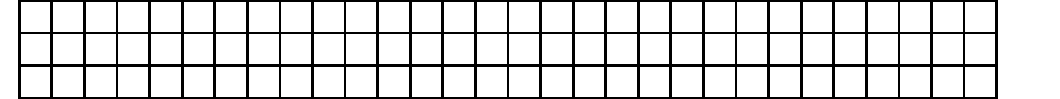
\includegraphics[scale=0.475]{Figures/beamMesh.pdf}
  \label{fig:vigaMesh}
  }
  \caption{Cantilever beam.}
  \label{fig:cantileverBeam}
\end{figure}

This problem is simulated considering three different loading-unloading cases, one static (Figure \autoref{fig:force_static}) and two dynamic (Figures \autoref{fig:force_dynamic1} and \autoref{fig:force_dynamic2}) with material density $\rho=8000 \text{ kg}/\text{m}^3$ and time increment $\Delta t = 0.25 \text{ ms}$.
In \autoref{fig:beamStatic}, we compare the obtained displacement at the end of the beam to results from ANSYS for the static case. 
One can see that the analysis coincides with the reference until the end of the second loading cycle, when, possibly, the different strain measures used in the two analyzes affect the problem solution.
Finally, \autoref{fig:beamDynamic} shows the displacements magnitude over the simulated time for the dynamic cases, and the obtained results are in good agreement with te reference.


\begin{figure}[h]
  \centering 
  \subfigure[static case]{
  \includegraphics[scale=0.65]{Figures/graphs/force_static.pdf}
  \label{fig:force_static}
  }
  \subfigure[dynamic case 1]{
  \includegraphics[scale=0.65]{Figures/graphs/force_dynamic1.pdf}
  \label{fig:force_dynamic1}
  }
  \subfigure[dynamic case 2]{
    \includegraphics[scale=0.65]{Figures/graphs/force_dynamic2.pdf}
    \label{fig:force_dynamic2}
  }
  \caption{Simulated loading-unloading.}
  \label{fig:force}
\end{figure}

\begin{figure}[h]
  \centering 
  \includegraphics[scale=0.65]{Figures/graphs/beam_static.pdf}
  \caption{Force-displacement magnitude diagram for the static case.}
  \label{fig:beamStatic}
\end{figure}



\begin{figure}[h]
  \centering 
  \subfigure[case 1]{
  \includegraphics[scale=0.65]{Figures/graphs/beam_dynamic1.pdf}
  \label{fig:dispDynamic1}
  }
  \subfigure[case 2]{
  \includegraphics[scale=0.65]{Figures/graphs/beam_dynamic2.pdf}
  \label{fig:dispDynamic2}
  }
  \caption{Displacements magnitude versus time for the dynamic cases.}
  \label{fig:beamDynamic}
\end{figure}



% --------------------------------------------------------------------------
\section{Conclusions}\label{sec:conclusion}
% --------------------------------------------------------------------------

In this work, we present and implement a numerical approach for 2D modeling of elasto-plastic solids at large displacements and small/moderate strains, considering plane strain.
Such approach considers only linear isotropic hardening, but a perfect elasto-plastic material model can also be considered making $K_p = 0$, so that the developed computational code is able to simulate a large number of engineering problems.
The proposed formulation allows conserving NURBS geometric representation from design, which allows to simulate complex geometry problems without the need for a well-defined mesh. 
In this sense, the resulting computational program has been applied to simulate a cantilever beam subjected to static and dynamic load.
As can be seen in \autoref{sec:example}, good correspondence between the obtained results with the results of the ANSYS program is observed throughout the plasticity phenomenon.


% %-------------------------------------------------------------------------
\vspace{20pt}
\noindent \textbf{Acknowledgements.} 
The authors would like to acknowledge the Brazilian agency National Council for Scientific and Technological Development (CNPq) and the \textit{Coordenação de Aperfeiçoamento de Nível Superior} (CAPES) for the financial support given to this research.
\vspace{12pt}

% %--------------------------------------------------------------------------
\noindent \textbf{Authorship statement.} 
The authors hereby confirm that they are the sole liable persons responsible for the authorship of this work, and that all material that has been herein included as part of the present paper is either the property (and authorship) of the authors, or has the permission of the owners to be included here. 

\bibliography{bibliography}

\end{document}
% --------------------------------------------------------------------------
